\newpage
\section{Revisão da Teoria}

\subsection{Modulação Delta}

A modulação Delta usa L=2, ou seja, apenas 1 bit faz todo a codificação do sinal.
Essa codificação é extremamente eficiente pois não necessita de bits de sincronismo, ou de framing para a transmissão, permitindo uma comunicação a uma taxa mais baixa ainda. O sinal Delta modulado, sendo uma série de “1” e “0”, é uma sequência de impulsos espaçados de Ts. 
Em DM usa-se um estimador de primeira ordem, que é, apenas um delay de TS. Para demodular o sinal, necessita-se de um circuito integrador, sendo que o estimador é apenas um delay.
A função do receptor é a de acumular o sinal recebido. O somador e a linha de delay mostradas na figura acima podem ser substituídos por um simples circuito
integrador.
O transmissor também é igual ao da figura \ref{fig:modulador}, porém com um delay servindo como estimador. O circuito do transmissor também pode ser simplificado com o uso de simples integradores RC.
\begin{figure}[H]
    \centering
    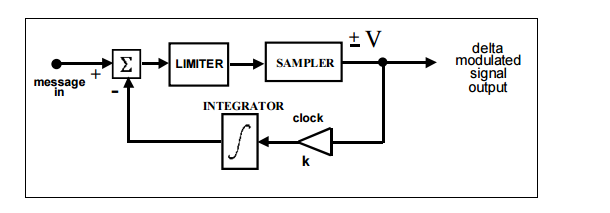
\includegraphics[scale=0.7]{modulador}
    \caption{Modulador delta.}
    \label{fig:modulador}
\end{figure}

Em PCM, o sinal analógico é quantizado em L níveis e essa informação é transmitida por n pulsos por amostra (n = Log2L). A diferença é que em DM o sinal
modulado não carrega informação sobre o sinal m(t) propriamente dito, mas sobre a sua derivada. Por isso dá-se este nome a essa modulação, delta modulation.
A grande vantagem do DM é que a modulação é feita em apenas 1 bit por amostra. Enquanto em PCM, normalmente há a necessidade de mais bits para codificar a amostra. A figura \ref{fig:saidadelta} mostra um exemplo da modulação de um sinal senoidal.

\begin{figure}[H]
    \centering
    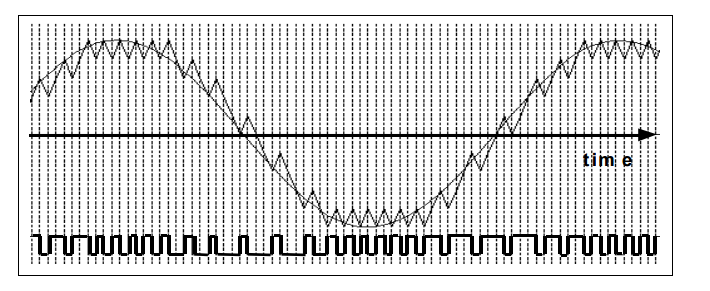
\includegraphics[scale=0.5]{saidadelta}
    \caption{Sinal senoidal com modulação delta.}
    \label{fig:saidadelta}
\end{figure}

\section{Diagrama de olho}

A técnica de medida conhecida como ‘diagrama de olho’, feita no domínio do tempo, é
uma ferramenta importante para se avaliar o desempenho de um sistema óptico digital, pois permite uma visualização da distorção na forma do sinal transmitido. Para se entender como o padrão do ‘olho’ é formado mostramos oito combinações de sinal NRZ com comprimento de 3-bit que, quando superpostas simultaneamente, formam um padrão de olho.

Algumas informações que podem ser obtidas com o diagrama do olho são (fonte: Mônica de Lacerda Rocha, Diagrama do olho. Projeto e avaliação Sistêmicos):

\begin{itemize}
    \item  A largura da abertura do olho (no eixo horizontal) define o intervalo de tempo sobre o qual o sinal recebido pode ser amostrado sem erro devido à interferência intersimbólica. O melhor momento de amostragem é o que corresponde ao de maior abertura vertical do olho.
    \item A altura da abertura do olho é reduzida quando ocorre distorção na amplitude do sinal. A distorção máxima é dada pela distância vertical entre o topo da abertura do olho e o
    máximo nível do sinal. Quanto mais fechado o olho se tornar, mais difícil é a detecção do sinal.

    \item A taxa na qual o olho se fecha, quando o instante de amostragem varia (i.e., proporcional à inclinação dos lados do diagrama de olho) determina a sensibilidade do sistema a erros de temporização. A probabilidade de ocorrência deste tipo de erro aumenta à medida que a inclinação torna-se mais acentuada.
    \item Jitter temporal (também conhecido como eixo de jitter ou 'distorção de fase') aparece devido ao ruído no receptor e à distorção do pulso na fibra. Se o sinal é amostrado no meio do intervalo de tempo de amostragem (i.e., eqüidistante entre os tempos de cruzamento do sinal com o nível de limiar), a distorção temporal, $\Delta T$, no nível de limiar indica a quantidade de jitter presente no sinal.
\end{itemize}

A figura \ref{fig:eyediagram} mostra o formato do diagrama do olho.

\begin{figure}[H]
    \centering
    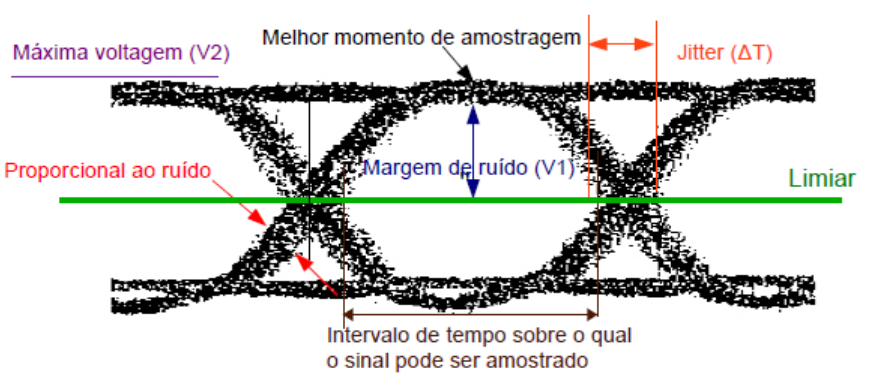
\includegraphics[scale=0.5]{eyediagram}
    \caption{Diagrama do olho.}
    \label{fig:eyediagram}
\end{figure}